\section{Introduction aux graphes}

\subsection{Vocabulaire des graphes}

\begin{defi}{Graphe}%\cite{ref_01}
Un graphe est un ensemble de \textbf{sommets} et  \textbf{relations} entre ces sommets.

Lorsque deux sommets sont en relation, on dit qu'il existe une \textbf{arête} entre ces sommets.
\end{defi}

\begin{defi}{Graphe non orienté -- Arêtes}
Un graphe non orienté $G$ est un couple $G=(S,A)$, où $S$ est un ensemble fini de sommets (appelés aussi n\oe uds)  et où $A$ est un ensemble fini de paires ordonnées de sommets, appelées arêtes.

On note $x - y$ l'arête $\{x,y\}$. $x$ et $y$ sont les deux extrémités de l'arête.
\end{defi}

\begin{defi}{Graphe orienté -- Arcs}\cite{ref_01}
Un graphe orienté $G$ est un couple $G=(S,A)$, où $S$ est un ensemble fini de sommets et où $A$ est un ensemble fini de paires ordonnées de sommets, appelées arcs.

On note $x\to y$ l'arc $(x,y)$. $x$ est l'extrémité initiale de l'arc, $y$ est son extrémité terminale. On dit que $y$ est successeur de $x$ et que $x$ est prédécesseur de $y$. 
\end{defi}

\begin{multicols}{2}
\begin{figure}[H]
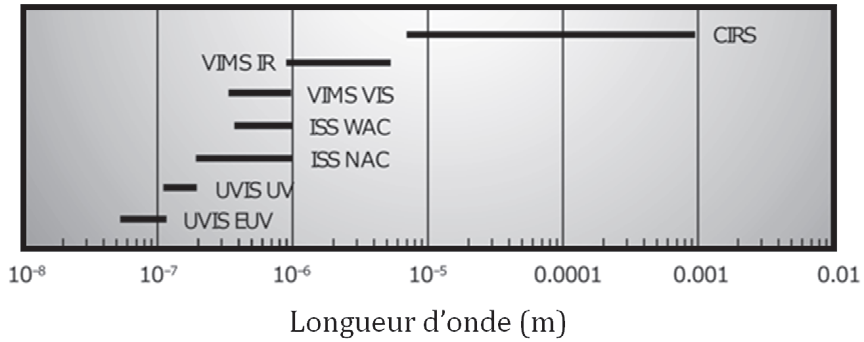
\includegraphics[width=.8\linewidth]{fig_02}
\captionsetup{justification=centering}
\caption{Graphe non orienté \label{fig_02}}
\end{figure}

\begin{figure}[H]
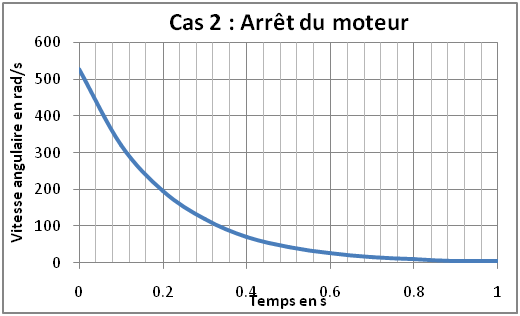
\includegraphics[width=.8\linewidth]{fig_03}
\captionsetup{justification=centering}
\caption{Graphe orienté}
\end{figure}
\end{multicols}


\begin{defi}{Adjacence}
Deux arcs (resp. arêtes) d'un graphe orienté (resp. non orienté) sont dits adjacents s'ils ont au moins une extrémité commune. 

Deux sommets d'un graphe non orienté sont dits adjacents s'il existe une arête les joignant. 

Dans un graphe orienté, le sommet $y$ est dit adjacent au sommet $x$ s'il existe un arc $x\to y$.
\end{defi}


\begin{defi}{Sommet (ou n\oe{}uds)}
\end{defi}

\begin{defi}{Arc, arête}
\end{defi}

\begin{defi}{Chemin d'un sommet à un autre}
\end{defi}

\begin{defi}{Cycle}
\end{defi}

\begin{defi}{Connexité dans les graphes non orientés}
\end{defi}

\subsection{Notations}
\begin{defi}{Degré d'un sommet}
On appelle degré d'un sommet $s$ et on note $d\left(s\right)$ le nombres d'arcs (ou d'arêtes) dont $s$ est une extrémité.
\end{defi}

\begin{defi}{Degré entrant et sortant}
On note $s$ le sommet d'un graphe orienté. On note : 
\begin{itemize}
\item $d_{+}\left(s\right)$ le demi-degré extérieur de $s$, c'est-à-dire le nombre d'arcs ayant leur extrémité initiale en $s$ (ces arcs sont dits incidents à $s$ vers l'extérieur);
\item $d_{-}\left(s\right)$ le demi-degré intérieur de $s$, c'est-à-dire le nombre d'arcs ayant leur extrémité finale en $s$ (ces arcs sont dits incidents à $s$ vers l'intérieur).
\end{itemize}

Dans ce cas, on a  $d\degres\left(s\right)=d_{-}\left(s\right)+d_{+}\left(s\right)$.
\end{defi}


\begin{exemple}~\\

\begin{multicols}{2}
\begin{figure}[H]
\centering
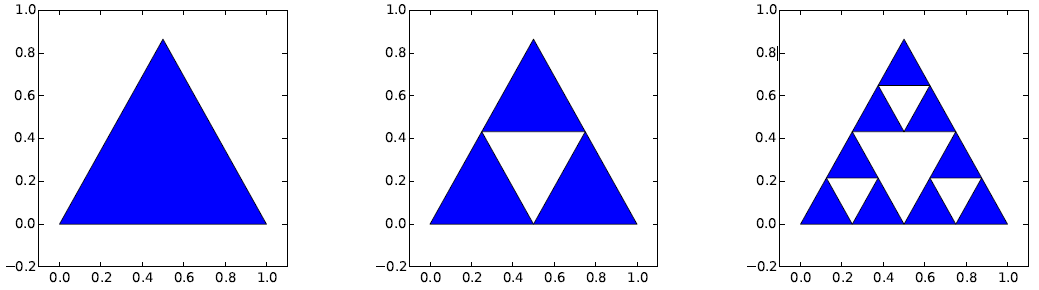
\includegraphics[width=.8\linewidth]{fig_04}
\captionsetup{justification=centering}
\caption{Graphe orienté \label{fig_04}}
\end{figure}

\begin{itemize}
\item $d_{-}\left(S_1\right)=3$.
\item $d_{+}\left(S_1\right)=4$.
\item $d\degres\left(S_1\right)=7$.
\end{itemize}
\end{multicols}

\end{exemple}

\subsection{Implémentation des graphes}

\subsubsection{Liste d'adjacence}

\subsubsection{Matrice d'adjacence}



\section{Parcours d'un graphe}
\subsection{Piles et files}

\subsection{Parcours générique d'un graphe}

\subsection{Parcours en largeur}

\subsection{Parcours en profondeur}

\subsection{Détection de la présence des cycles}

\subsection{Connexité d'un graphe non orienté}

\section{Pondération d'un graphe}



\section{Recheche du plus court chemin}
\subsection{Algorithme de Dijkstra}

\subsection{Algorithme A$\star$}

\begin{defi}{}
\end{defi}

\begin{defi}{}
\end{defi}

\begin{defi}{}
\end{defi}

\begin{defi}{}
\end{defi}

\begin{defi}{}
\end{defi}
